\documentclass{article}
\usepackage[utf8]{inputenc}
\usepackage{hyperref}
\usepackage{color}
\usepackage{tikzsymbols}
\usepackage{subfig}
\usepackage{graphicx}
\usepackage{blindtext}

\title{Report :: TIPR Assignment - II}
\author{Prasanna Patil}
\date{4 March, 2018}

\begin{document}

\maketitle
\section{Configuration}
\begin{itemize}
	\item Python code is written for Python 3. It may not work with Python 2.
	\item The Cat-Dog images were rescaled to (28, 28) resolution and model was trained on grayscale images.
	\item The code should be executed from within src folder, otherwise relative paths may not work as expected.
	\item Two datasets are recognized as "MNIST" and "Cat-Dog" (without quotes).
	\item Pass the configuration as a string list. That is, argument should be --configuration '[30 10]' (\textbf{with} quotes).
\end{itemize}

\section{Part 1:- MNIST}
\subsection{Task 1:- Test Model with different number of layers}
Tested model with single, double and triple layers. Each having 30 number of neurons. Following plots show the various metrics for different layers.

\begin{figure}[!htb]
	\minipage{0.5\textwidth}
	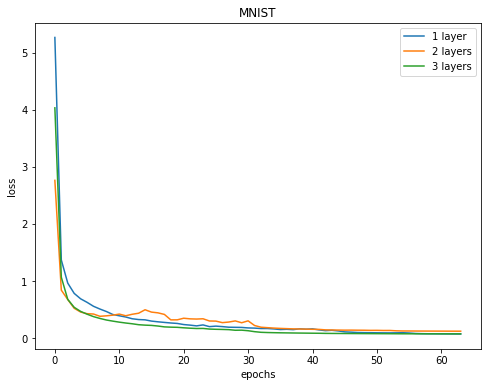
\includegraphics[width=\linewidth]{../output_plots/part_1_task_1_loss.png}
	\caption{Loss}\label{fig:part_1_task_1_loss}
	\endminipage\hfill
	\minipage{0.5\textwidth}
	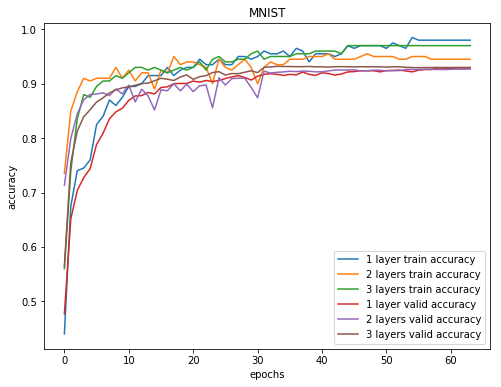
\includegraphics[width=\linewidth]{../output_plots/part_1_task_1_accuracy.png}
	\caption{Accuracy}\label{fig:part_1_task_1_accuracy}
	\endminipage\hfill
	\minipage{0.5\textwidth}%
	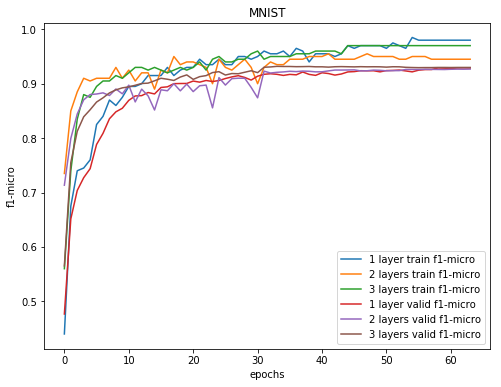
\includegraphics[width=\linewidth]{../output_plots/part_1_task_1_f1-micro.png}
	\caption{F1-Micro}\label{fig:part_1_task_1_f1-micro}
	\endminipage
	\minipage{0.5\textwidth}%
	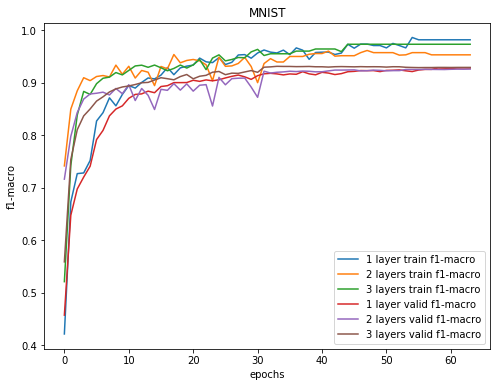
\includegraphics[width=\linewidth]{../output_plots/part_1_task_1_f1-macro.png}
	\caption{F1-Macro}\label{fig:part_1_task_1_f1-macro}
	\endminipage
\end{figure}

Each plot shows the metric on Y-axis and epochs on X-axis. Different lines in plot corresponds to different models.

\subsection{Task 2:- Test Model with different number of neurons and layers}

Tested model with following configurations:
\begin{itemize}
	\item 784-50-10
	\item 785-50-30-10
	\item784-100-10
	\item 784-50-50-30-10
\end{itemize}

Finally fixed and fine-tuned the 784-50-30-10 model as it took less time for training and had comparable performance.

\begin{figure}[!htb]
	\minipage{0.5\textwidth}
	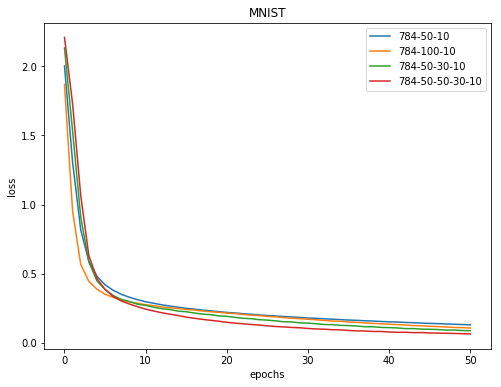
\includegraphics[width=\linewidth]{../output_plots/part_1_task_2_loss.png}
	\caption{Loss}\label{fig:part_1_task_2_loss}
	\endminipage\hfill
	\minipage{0.5\textwidth}
	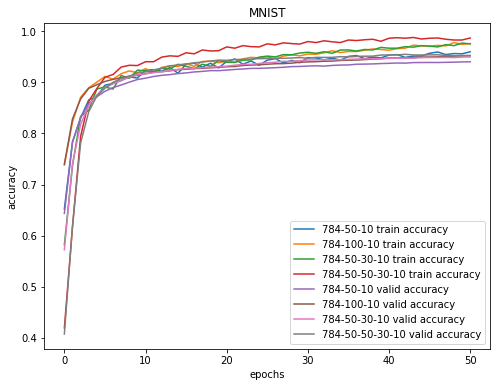
\includegraphics[width=\linewidth]{../output_plots/part_1_task_2_accuracy.png}
	\caption{Accuracy}\label{fig:part_1_task_2_accuracy}
	\endminipage\hfill
	\minipage{0.5\textwidth}%
	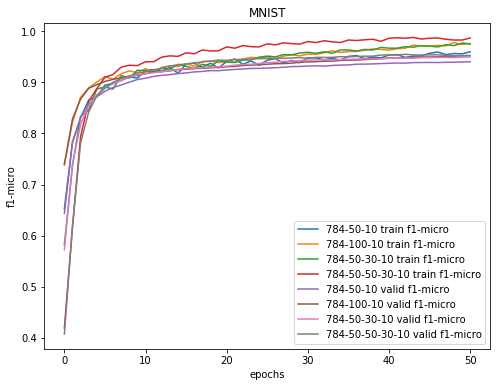
\includegraphics[width=\linewidth]{../output_plots/part_1_task_2_f1-micro.png}
	\caption{F1-Micro}\label{fig:part_1_task_2_f1-micro}
	\endminipage
	\minipage{0.5\textwidth}%
	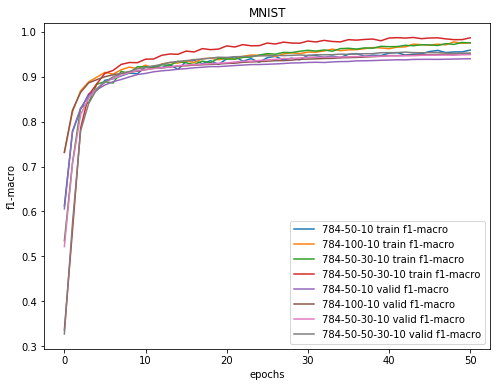
\includegraphics[width=\linewidth]{../output_plots/part_1_task_2_f1-macro.png}
	\caption{F1-Macro}\label{fig:part_1_task_2_f1-macro}
	\endminipage
\end{figure}

Each plot shows the metric on Y-axis and epochs on X-axis. Different lines in plot corresponds to different models.

\subsection{Task 3:- Test Model with different activation functions}

Tested model with relu, tanh, sigmoid and swish activations functions. The performance of relu and swish were almost same and decided to use swish in the final model. For grayscale images tanh performed better than sigmoid in convergence rate.

\begin{figure}[!htb]
	\minipage{0.5\textwidth}
	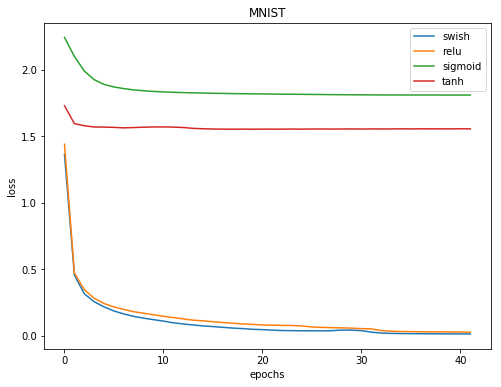
\includegraphics[width=\linewidth]{../output_plots/part_1_task_3_loss.png}
	\caption{Loss}\label{fig:part_1_task_3_loss}
	\endminipage\hfill
	\minipage{0.5\textwidth}
	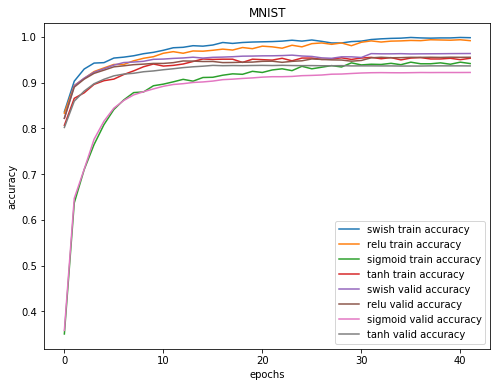
\includegraphics[width=\linewidth]{../output_plots/part_1_task_3_accuracy.png}
	\caption{Accuracy}\label{fig:part_1_task_3_accuracy}
	\endminipage\hfill
	\minipage{0.5\textwidth}
	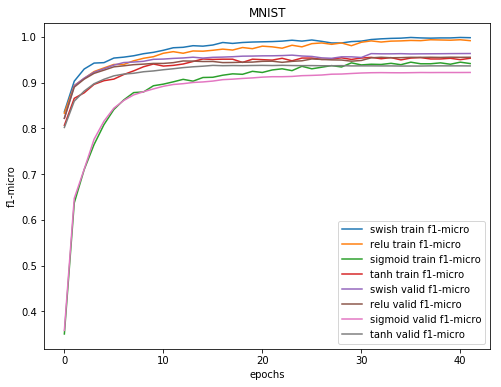
\includegraphics[width=\linewidth]{../output_plots/part_1_task_3_f1-micro.png}
	\caption{F1-Micro}\label{fig:part_1_task_3_f1-micro}
	\endminipage
	\minipage{0.5\textwidth}
	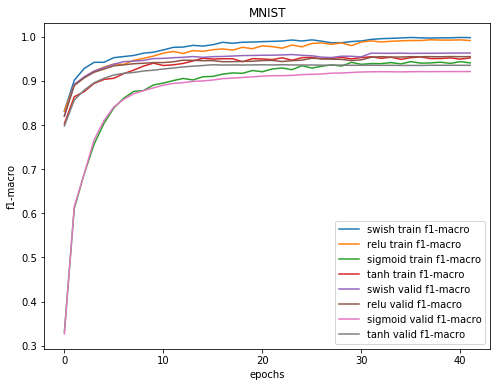
\includegraphics[width=\linewidth]{../output_plots/part_1_task_3_f1-macro.png}
	\caption{F1-Macro}\label{fig:part_1_task_3_f1-macro}
	\endminipage
\end{figure}

Each plot shows the metric on Y-axis and epochs on X-axis. Different lines in plot corresponds to different models.

\pagebreak

\subsection{Task 4:- Run Model with Keras code}

Tested the same models as in above tasks but this time used keras to implement the Feed Forward Network.

\subsubsection{Testing with different Layers}

\begin{figure}[!htb]
	\minipage{0.5\textwidth}
	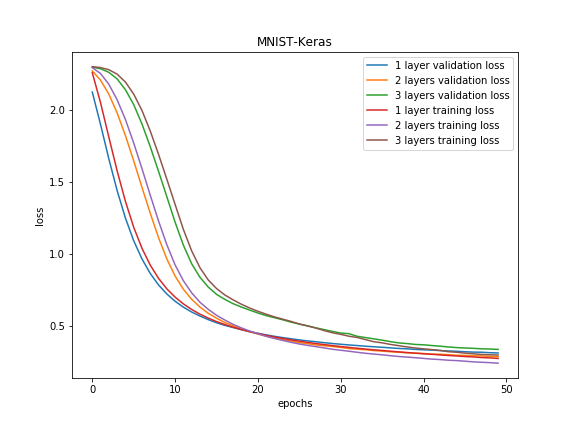
\includegraphics[width=\linewidth]{../output_plots/part_1_task_4_layers_loss.png}
	\caption{Loss}\label{fig:part_1_task_4_layers_loss}
	\endminipage\hfill
	\minipage{0.5\textwidth}
	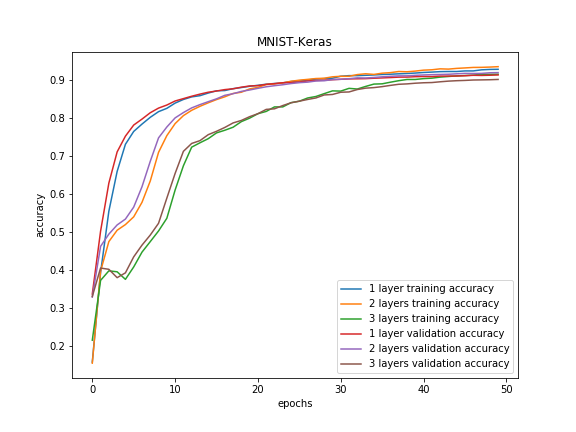
\includegraphics[width=\linewidth]{../output_plots/part_1_task_4_layers_accuracy.png}
	\caption{Accuracy}\label{fig:part_1_task_4_layers_accuracy}
	\endminipage\hfill
\end{figure}

\subsubsection{Testing with different architectures}

\begin{figure}[!htb]
	\minipage{0.5\textwidth}
	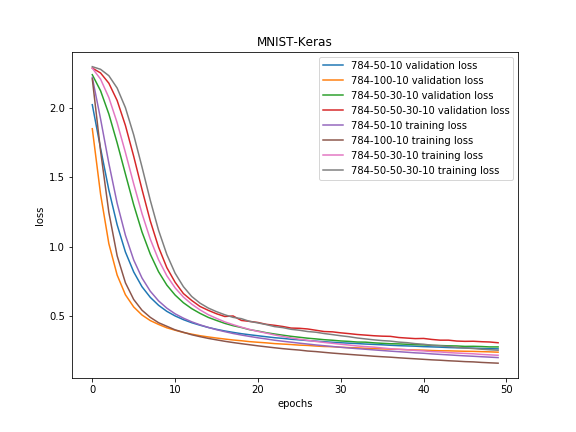
\includegraphics[width=\linewidth]{../output_plots/part_1_task_4_best_loss.png}
	\caption{Loss}\label{fig:part_1_task_4_best_loss}
	\endminipage\hfill
	\minipage{0.5\textwidth}
	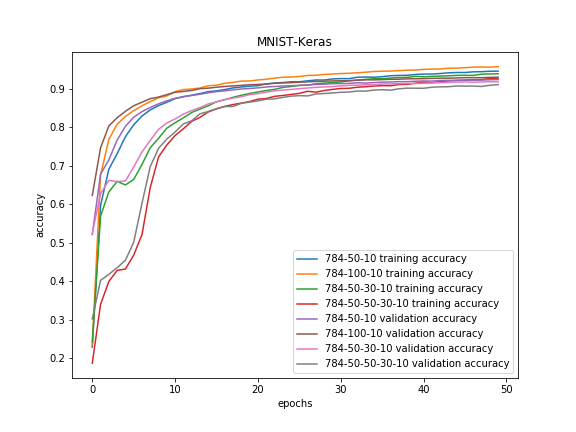
\includegraphics[width=\linewidth]{../output_plots/part_1_task_4_best_accuracy.png}
	\caption{Accuracy}\label{fig:part_1_task_4_best_accuracy}
	\endminipage\hfill
\end{figure}

\pagebreak
\subsubsection{Testing with different activation functions}

\begin{figure}[!htb]
	\minipage{0.5\textwidth}
	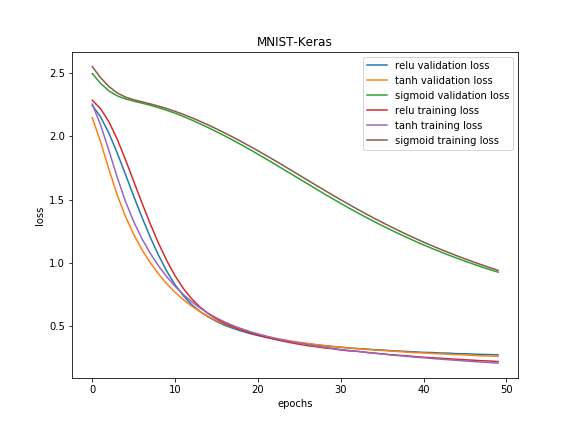
\includegraphics[width=\linewidth]{../output_plots/part_1_task_4_activations_loss.png}
	\caption{Loss}\label{fig:part_1_task_4_activations_loss}
	\endminipage\hfill
	\minipage{0.5\textwidth}
	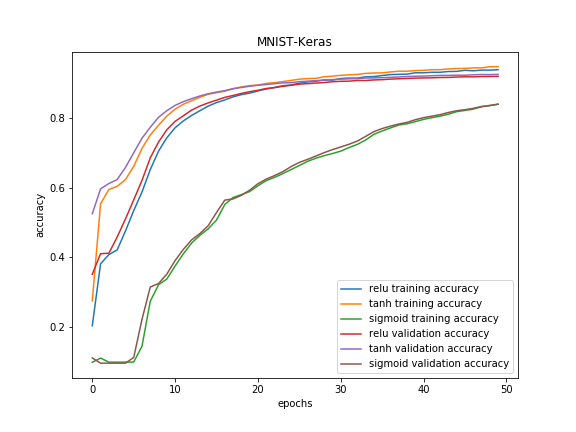
\includegraphics[width=\linewidth]{../output_plots/part_1_task_4_activations_accuracy.png}
	\caption{Accuracy}\label{fig:part_1_task_4_activations_accuracy}
	\endminipage\hfill
\end{figure}

\pagebreak

\section{Part 2:- Cat-Dog}
\subsection{Task 1:- Test Model with different number of layers}

Tested model with single, double and triple layers. Each having 200 number of neurons. Following plots show the various metrics for different layers.

\begin{figure}[!htb]
	\minipage{0.5\textwidth}
	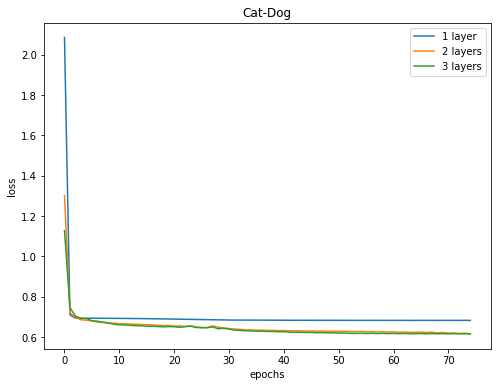
\includegraphics[width=\linewidth]{../output_plots/part_2_task_1_loss.png}
	\caption{Loss}\label{fig:part_2_task_1_loss}
	\endminipage\hfill
	\minipage{0.5\textwidth}
	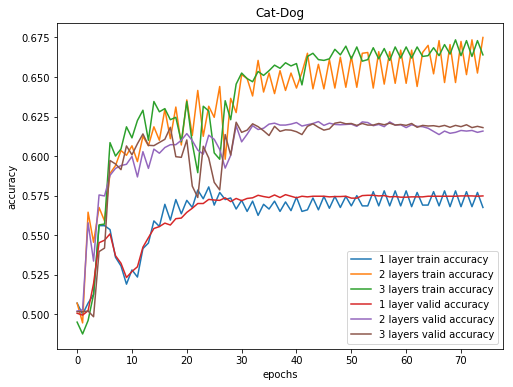
\includegraphics[width=\linewidth]{../output_plots/part_2_task_1_accuracy.png}
	\caption{Accuracy}\label{fig:part_2_task_1_accuracy}
	\endminipage\hfill
	\minipage{0.5\textwidth}%
	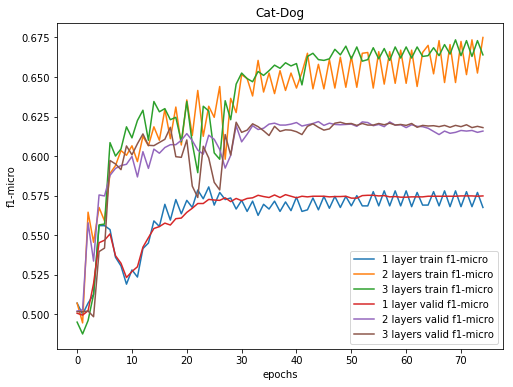
\includegraphics[width=\linewidth]{../output_plots/part_2_task_1_f1-micro.png}
	\caption{F1-Micro}\label{fig:part_2_task_1_f1-micro}
	\endminipage
	\minipage{0.5\textwidth}%
	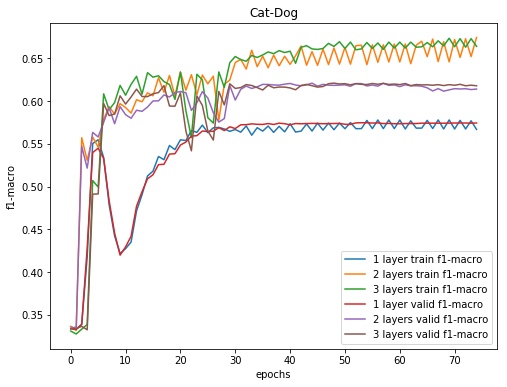
\includegraphics[width=\linewidth]{../output_plots/part_2_task_1_f1-macro.png}
	\caption{F1-Macro}\label{fig:part_2_task_1_f1-macro}
	\endminipage
\end{figure}

Each plot shows the metric on Y-axis and epochs on X-axis. Different lines in plot corresponds to different models.


\subsection{Task 2:- Test Model with different number of neurons and layers}

Tested model with following configurations:
\begin{itemize}
	\item 784-50-10
	\item 785-50-30-10
	\item784-100-10
	\item 784-50-50-30-10
\end{itemize}

Finally fixed and fine-tuned the 784-50-30-10 model as it took less time for training and had comparable performance.

\begin{figure}[!htb]
	\minipage{0.5\textwidth}
	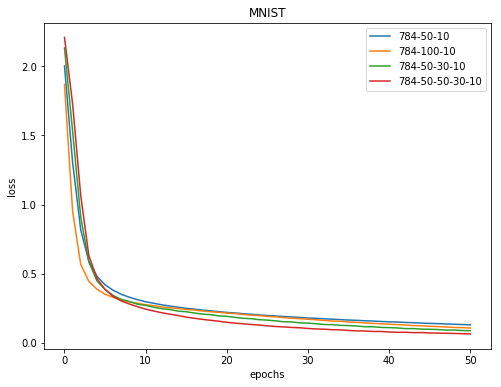
\includegraphics[width=\linewidth]{../output_plots/part_1_task_2_loss.png}
	\caption{Loss}\label{fig:part_1_task_2_loss}
	\endminipage\hfill
	\minipage{0.5\textwidth}
	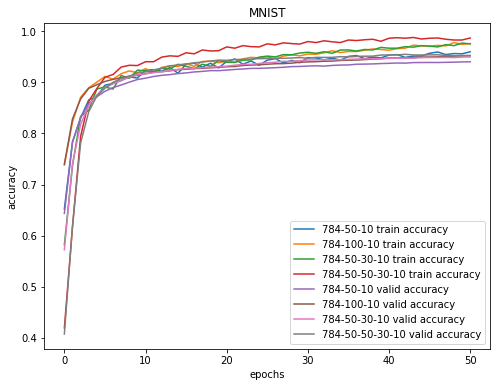
\includegraphics[width=\linewidth]{../output_plots/part_1_task_2_accuracy.png}
	\caption{Accuracy}\label{fig:part_1_task_2_accuracy}
	\endminipage\hfill
	\minipage{0.5\textwidth}%
	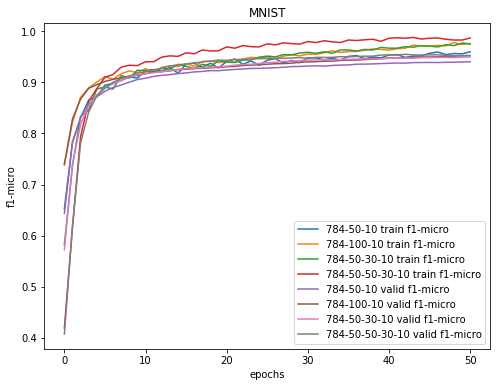
\includegraphics[width=\linewidth]{../output_plots/part_1_task_2_f1-micro.png}
	\caption{F1-Micro}\label{fig:part_1_task_2_f1-micro}
	\endminipage
	\minipage{0.5\textwidth}%
	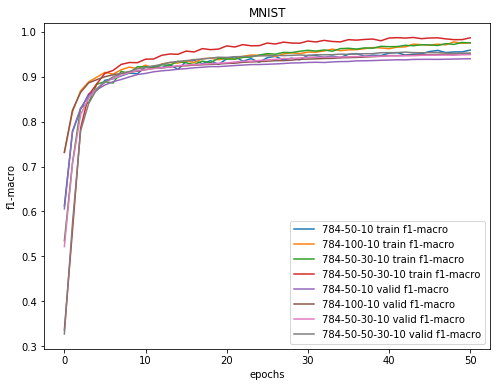
\includegraphics[width=\linewidth]{../output_plots/part_1_task_2_f1-macro.png}
	\caption{F1-Macro}\label{fig:part_1_task_2_f1-macro}
	\endminipage
\end{figure}

Each plot shows the metric on Y-axis and epochs on X-axis. Different lines in plot corresponds to different models.

\pagebreak
\subsection{Task 3:- Test Model with different activation functions}

Tested model with relu, tanh, sigmoid and swish activations functions. The performance of relu and swish were almost same and decided to use swish in the final model. For grayscale images tanh performed better than sigmoid in convergence rate.

\begin{figure}[!htb]
	\minipage{0.5\textwidth}
	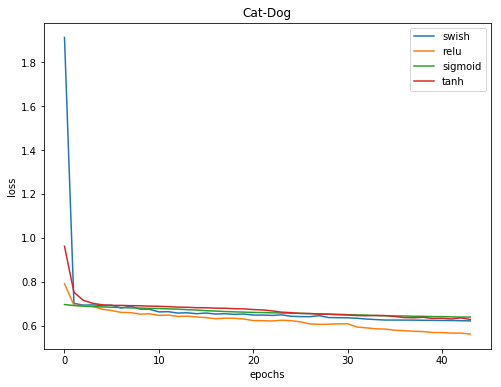
\includegraphics[width=\linewidth]{../output_plots/part_2_task_3_loss.png}
	\caption{Loss}\label{fig:part_2_task_3_loss}
	\endminipage\hfill
	\minipage{0.5\textwidth}
	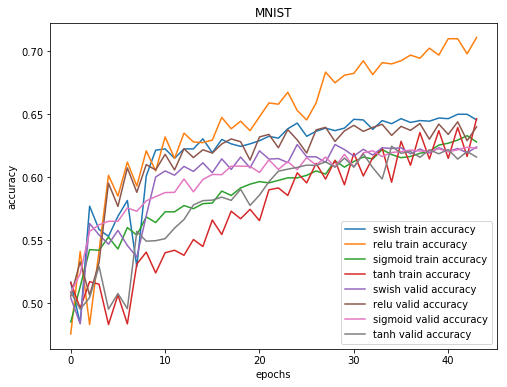
\includegraphics[width=\linewidth]{../output_plots/part_2_task_3_accuracy.png}
	\caption{Accuracy}\label{fig:part_2_task_3_accuracy}
	\endminipage\hfill
	\minipage{0.5\textwidth}
	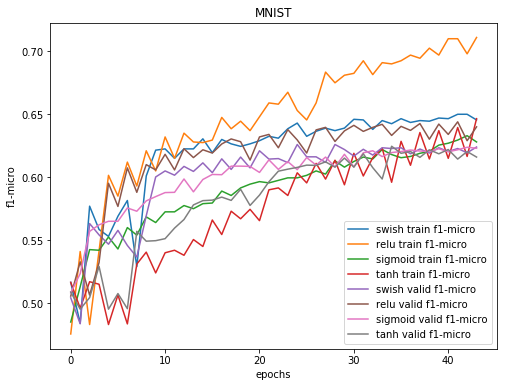
\includegraphics[width=\linewidth]{../output_plots/part_2_task_3_f1-micro.png}
	\caption{F1-Micro}\label{fig:part_2_task_3_f1-micro}
	\endminipage
	\minipage{0.5\textwidth}
	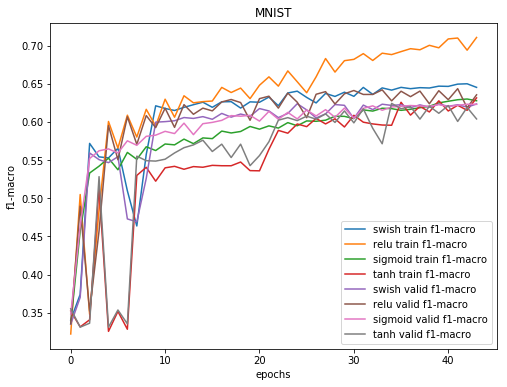
\includegraphics[width=\linewidth]{../output_plots/part_2_task_3_f1-macro.png}
	\caption{F1-Macro}\label{fig:part_2_task_3_f1-macro}
	\endminipage
\end{figure}

Each plot shows the metric on Y-axis and epochs on X-axis. Different lines in plot corresponds to different models.

\pagebreak
\subsection{Task 4:- Run Model with Keras code}
Tested the same models as in above tasks but this time used keras to implement the Feed Forward Network.

\subsubsection{Testing with different Layers}

\begin{figure}[!htb]
	\minipage{0.5\textwidth}
	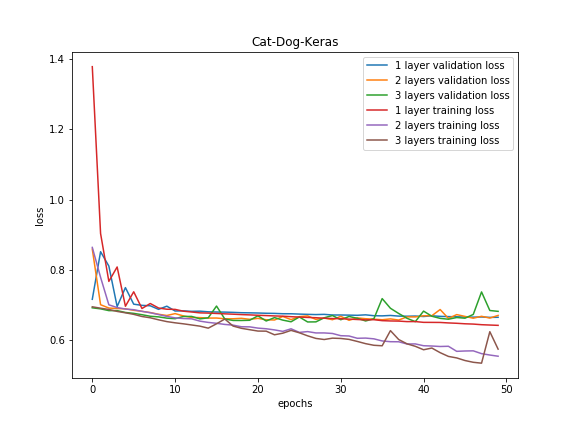
\includegraphics[width=\linewidth]{../output_plots/part_2_task_4_layers_loss.png}
	\caption{Loss}\label{fig:part_2_task_4_layers_loss}
	\endminipage\hfill
	\minipage{0.5\textwidth}
	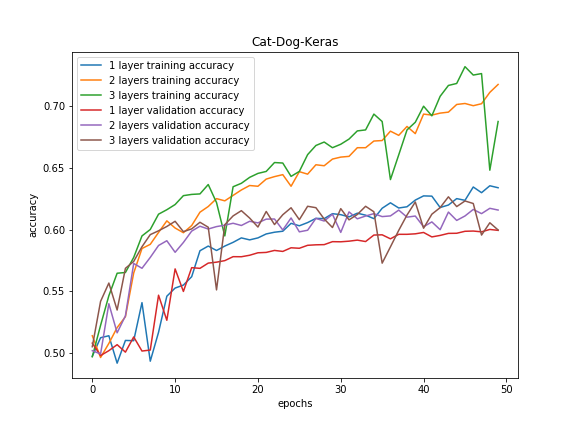
\includegraphics[width=\linewidth]{../output_plots/part_2_task_4_layers_accuracy.png}
	\caption{Accuracy}\label{fig:part_2_task_4_layers_accuracy}
	\endminipage\hfill
\end{figure}

\subsubsection{Testing with different architectures}

\begin{figure}[!htb]
	\minipage{0.5\textwidth}
	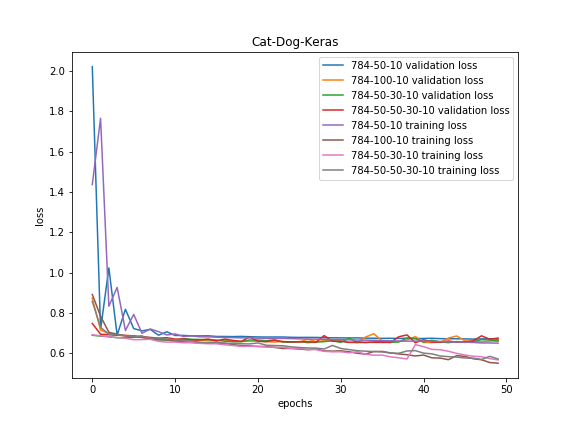
\includegraphics[width=\linewidth]{../output_plots/part_2_task_4_best_loss.png}
	\caption{Loss}\label{fig:part_2_task_4_best_loss}
	\endminipage\hfill
	\minipage{0.5\textwidth}
	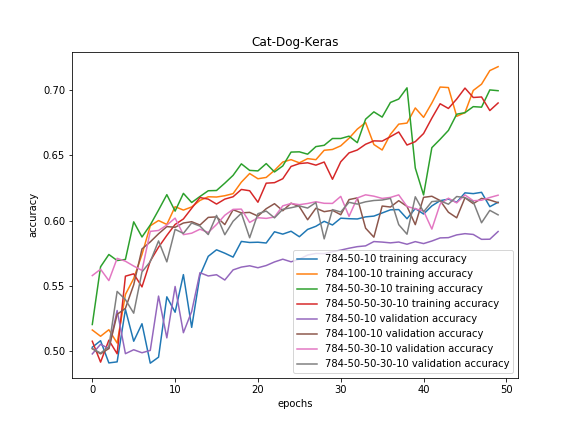
\includegraphics[width=\linewidth]{../output_plots/part_2_task_4_best_accuracy.png}
	\caption{Accuracy}\label{fig:part_2_task_4_best_accuracy}
	\endminipage\hfill
\end{figure}

\pagebreak
\subsubsection{Testing with different activation functions}

\begin{figure}[!htb]
	\minipage{0.5\textwidth}
	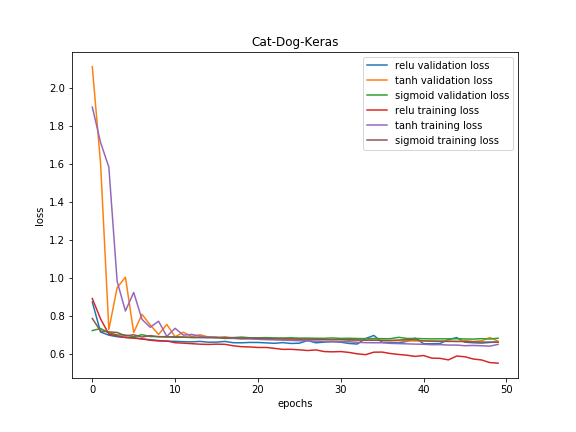
\includegraphics[width=\linewidth]{../output_plots/part_2_task_4_activations_loss.png}
	\caption{Loss}\label{fig:part_2_task_4_activations_loss}
	\endminipage\hfill
	\minipage{0.5\textwidth}
	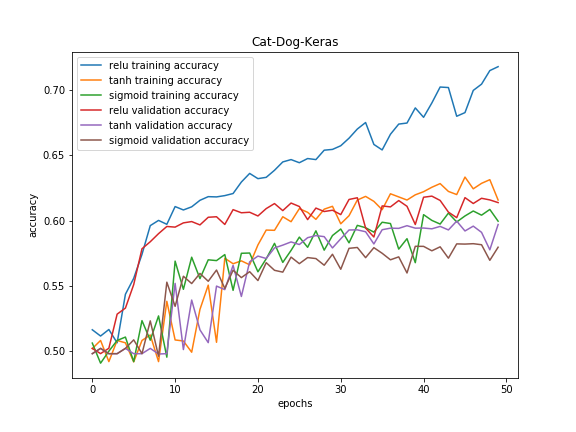
\includegraphics[width=\linewidth]{../output_plots/part_2_task_4_activations_accuracy.png}
	\caption{Accuracy}\label{fig:part_2_task_4_activations_accuracy}
	\endminipage\hfill
\end{figure}

\pagebreak
\section{Part 3:- Pubmed, Twitter and Dolphins}
\subsection{PubMed Dataset}
Following plot shows accuracy and loss when neural network was trained on pubmed dataset.

\begin{figure}[!htb]
	\minipage{0.5\textwidth}
	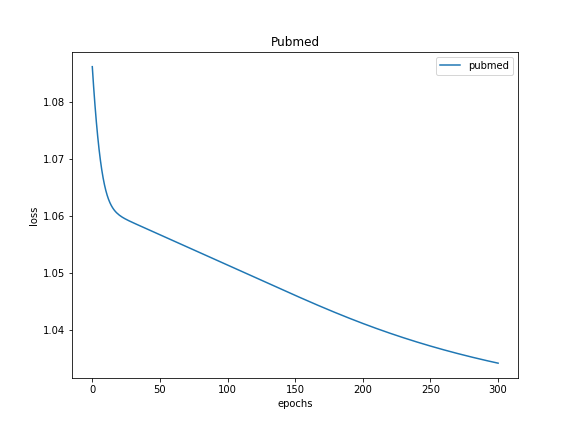
\includegraphics[width=\linewidth]{../output_plots/part_3_pubmed_loss.png}
	\caption{Loss}\label{fig:part_3_pubmed_loss}
	\endminipage\hfill
	\minipage{0.5\textwidth}
	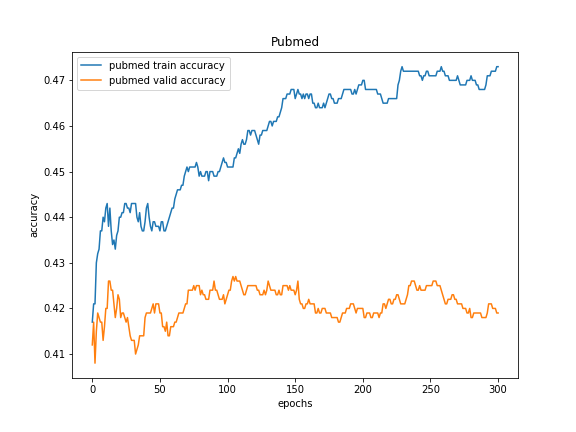
\includegraphics[width=\linewidth]{../output_plots/part_3_pubmed_accuracy.png}
	\caption{Accuracy}\label{fig:part_3_pubmed_accuracy}
	\endminipage\hfill
\end{figure}

\subsection{Twitter Dataset}
Following plot shows accuracy and loss when neural network was trained on twitter dataset.

\begin{figure}[!htb]
	\minipage{0.5\textwidth}
	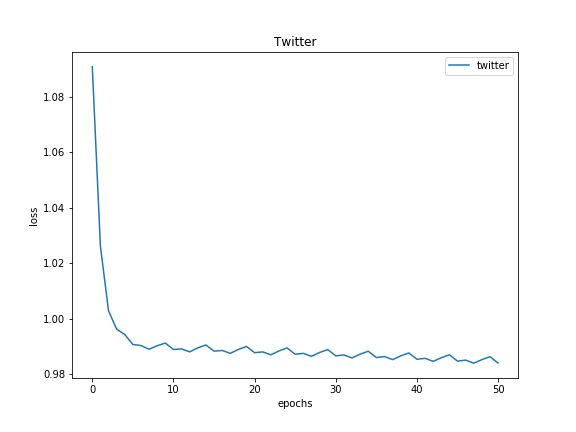
\includegraphics[width=\linewidth]{../output_plots/part_3_twitter_loss.png}
	\caption{Loss}\label{fig:part_3_twitter_loss}
	\endminipage\hfill
	\minipage{0.5\textwidth}
	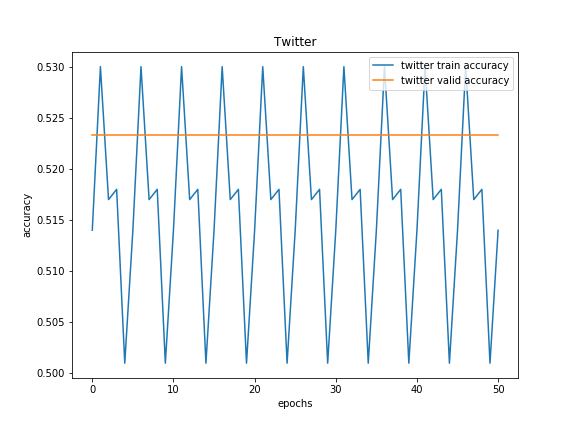
\includegraphics[width=\linewidth]{../output_plots/part_3_twitter_accuracy.png}
	\caption{Accuracy}\label{fig:part_3_twitter_accuracy}
	\endminipage\hfill
\end{figure}

\pagebreak
\subsection{Dolphins Dataset}
Following plot shows accuracy and loss when neural network was trained on dolphins dataset.

\begin{figure}[!htb]
	\minipage{0.5\textwidth}
	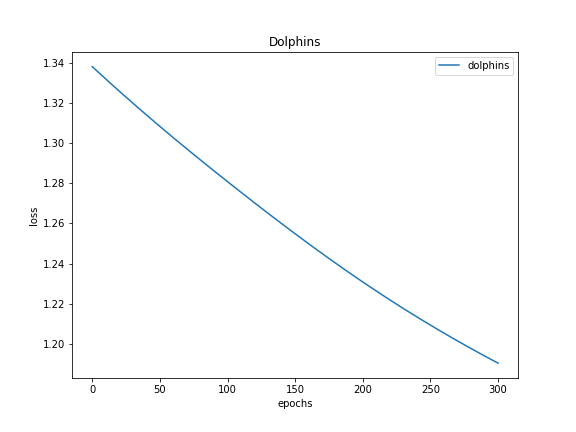
\includegraphics[width=\linewidth]{../output_plots/part_3_dolphins_loss.png}
	\caption{Loss}\label{fig:part_3_dolphins_loss}
	\endminipage\hfill
	\minipage{0.5\textwidth}
	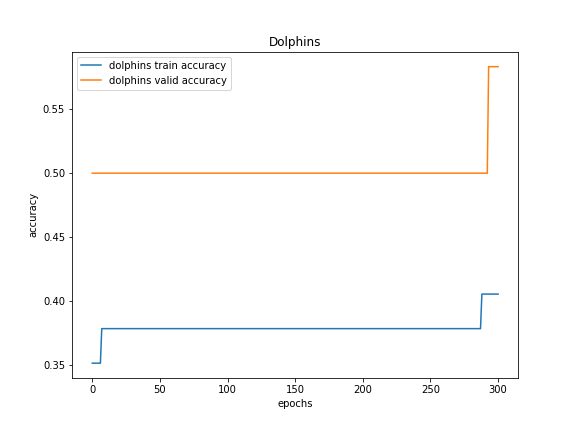
\includegraphics[width=\linewidth]{../output_plots/part_3_dolphins_accuracy.png}
	\caption{Accuracy}\label{fig:part_3_dolphins_accuracy}
	\endminipage\hfill
\end{figure}


\end{document}